%! Author = Len Washington III
%! Date = 9/12/2023

% Preamble
\documentclass[12pt]{report}

% Packages
\usepackage[11]{cs430lecture}

% Document
\begin{document}

%<*Lecture-Activity-11>
\tikzset{every tree node/.style={minimum width=2em,draw,circle},
         blank/.style={draw=none},
         edge from parent/.style=
         {draw,edge from parent path={(\tikzparentnode) -- (\tikzchildnode)}},
         level distance=1cm}
\section{Opening Questions}\label{sec:opening-questions-11}
\begin{enumerate}[label=\arabic*.]
    \item What is the main problem with Binary Search Trees that Red-Black Trees correct? Explain briefly (2--3 sentences) how Red-Black Trees correct this problem with Binary Search Trees. \answer{The biggest problem is that the tree may be a straight line that would cause the height to be $O(n)$. Red-Black trees maintain this balance by keeping track of the colors and allows the tree to be better balanced using a \hyperref[dfn:red-black-tree-properties]{specific set of rules}.}
	\item For the balanced binary search trees, why is it important that we can show that a rotation at a node is $O(1)$ (i.e. not dependent on the size of the BST) \answer{We want to make fixes that are not dependent on the size of a binary tree.}
\end{enumerate}

\section{Red-Black Trees}\label{sec:red-black-trees}
Red-Black Properties
\begin{enumerate}[label=\arabic*.]\label{dfn:red-black-tree-properties}
    \item\label{itm:red-black-tree-property1} Every node is colored either red or black
	\item\label{itm:red-black-tree-property2} The root is black
	\item\label{itm:red-black-tree-property3} Every null pointer descending from a leaf is considered to be a null black leaf node
	\item\label{itm:red-black-tree-property4} If a node is red, then both of its children are black
	\item\label{itm:red-black-tree-property5} For each node, all paths from the node to descendant leaves contain the same number of black nodes (\hyperref[dfn:black-height]{black height})
\end{enumerate}

\answer{
	\begin{tikzpicture} % TODO: Finish this tree
		\Tree
		[.$5$
			[.$3$
				[.$1$
					[.null ]
					[.null ]
				]
				[.$4$
					[.null ]
					[.null ]
				]
			]
			[.$8$
				[.null ]
				[.$12$
					[.null ]
					[.$15$ ]
				]
		]]
		\end{tikzpicture}}

black-height of a node\label{dfn:black-height} $bh(x)$ -- The number of black nodes on any path from, but not including, a node $x$ down to a null black leaf node. \answer{(Black height counts black nodes including null leaves, height doesn't count null nodes.)}
\begin{enumerate}[label=\arabic*.]
    \item If a node $x$ has $bh(x)=3$, what is its largest and smallest possible height (distance to the farthest leaf) in the BST? \answer{2--5}
	\item Prove using induction and red-black tree properties. A red-black tree with $n$ internal nodes \answer{(nodes with values), none null nodes} ($n$ key values) has height at most $2\lg(n+1)$
	\begin{enumerate}[label=Part \Alph*)]
	    \item\label{prb:2a} First show the sub-tree rooted at node $x$ has at least $2^{bh(x)}-1$ internal nodes. Use induction. \answer{Relating the black height of a node to how many values at least must be in that subtree.\\
		\textbf{Base Case}: $bh(x)=0$  \\\tikzset{every tree node/.style={minimum width=2em,draw,circle},
         blank/.style={draw=none},
         edge from parent/.style=
         {draw,edge from parent path={(\tikzparentnode) -- (\tikzchildnode)}},
         level distance=2cm}\begin{tikzpicture}
		\Tree
		[.Root~$x$
			[.null ]
		]
		\end{tikzpicture}\\ This tree has $bh=1$, with the only internal node being the root. \begin{equation*}
		\begin{aligned}
			2^{\mbox{bh(x)}} - 1 &= 2^{0} - 1\\
								 &= 1 - 1\\
								 &= 0\\
		\end{aligned}
		\end{equation*}
		\textbf{Induction Step}: Assuming at least $2^{bh(x)}-1$ keys in some subtree rooted at $x$.\\If a node is \textcolor{red}{red}, $bh(\mbox(parent)) = bh(\mbox(child))$ else a node is \textcolor{black}{black}, then the $bh(\mbox(parent)) = bh(\mbox(child))+1$.\begin{equation*}
		\begin{aligned}
			\left( 2^{bh(x)} - 1 \right) \left( 2^{bh(x)} - 1 \right) + 1 &= 2 \times \left( 2^{bh(x)} - 1 \right) + 1\\
		\end{aligned}
		\end{equation*}
		}
		\item Let $h$ be height of a Red-Black Tree, by \hyperref[itm:red-black-tree-property4]{property four}, at least half of the nodes on path from root to leaf are black \[ bh(root) \geq \frac{h}{2} \] Use that and \hyperref[prb:2a]{Part A} to show \[ h \leq 2\log(n+1) \] \answer{$bh(root)=k$ at least $2^{k}-1$.\begin{equation*}
		\begin{aligned}
			2^{bh(root)} - 1 &\leq n\\
			2^{h/2} - 1 &\leq n\\
			2^{h/2} &\leq n + 1\\
			\frac{h}{2} &\leq \lg(n + 1)\\
			h &\leq 2\lg(n + 1)\\
			h &= O(\lg(n + 1))\\
		\end{aligned}
		\end{equation*}}
	\end{enumerate}
	\item Which BST operations change for a red-black tree and which do not change? What do the operations that change need to be aware of and why?
	\begin{itemize}
		\item Search -- \answer{Won't change, you'd ignore the colors}
		\item \hyperref[alg:bst-insert]{Insert} -- \answer{Update}
		\item \hyperref[alg:bst-delete]{Delete} -- \answer{Update}
		\item Predecessor -- \answer{Won't change}
		\item \hyperref[alg:bst-successor]{Successor} -- \answer{Won't change} % TODO: Check if he said the runtime changes or the code changes
		\item Minimum -- \answer{Won't change}
		\item \hyperref[alg:extractmax]{Maximum} -- \answer{Won't change}
		\item \hyperref[alg:bst-left-rotate]{Rotations} -- \answer{Update}
	\end{itemize}
\end{enumerate}

\section{Red-Black Tree Insert}\label{sec:red-black-tree-insert} Similar to \hyperref[alg:bst-insert]{BST Insert}, assume we start with a valid red-black tree.
\begin{enumerate}[label=\arabic*.]
    \item Locate leaf position to insert new node
	\item Color new node red and create 2 new black null leafs below newly inserted red node
	\item If parent of new insert was \_\_\_\_\_\_\_\_\_\_ (fill in the blank, black or red), then done. ELSE procedure to recolor nodes and perform rotations to maintain red-black-properties.
\end{enumerate}

There are three cases if \hyperref[itm:red-black-tree-property4]{Red-Black Property \#4} when insert a red node $Z$ (or changed color of a node to red) and its parent is also red.\\

\begin{minipage}{0.45\textwidth}
	 \begin{figure}[H]
		 \centering
		 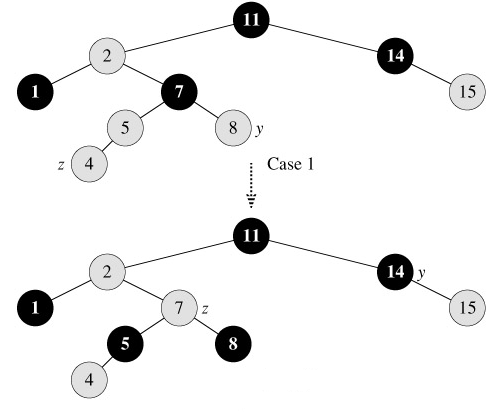
\includegraphics[width=\textwidth]{11.1}
		 \caption{Broken \hyperref[itm:red-black-tree-property4]{Red-Black Property \#4}: Case \#1}
		 \label{fig:red-black-insert-case-1}
	 \end{figure}
\end{minipage}\hfill
\begin{minipage}{0.5\textwidth}
	Node $Z$ (red) is a left or right child and its parent is red and its uncle is red (the children of nodes value $4$ $5$ $8$ must all be black, or null black).\\
	Swap the colors of a parent node and both its children, preserving the black height property at all nodes.
	\begin{itemize}
		\item Change $Z$'s parent and uncle to black
		\item Change $Z$'s grandparent to red
		\item No effect on black height on any node
		\item $Z$'s grandparent is now $Z$ and check again for \hyperref[itm:red-black-tree-property4]{property \#4} (two reds in a row) still broken at new node $Z$ (possible non-terminal case, need loop or recursion)
	\end{itemize}
\end{minipage}\\\\
\begin{minipage}{0.45\textwidth}
	 \begin{figure}[H]
		 \centering
		 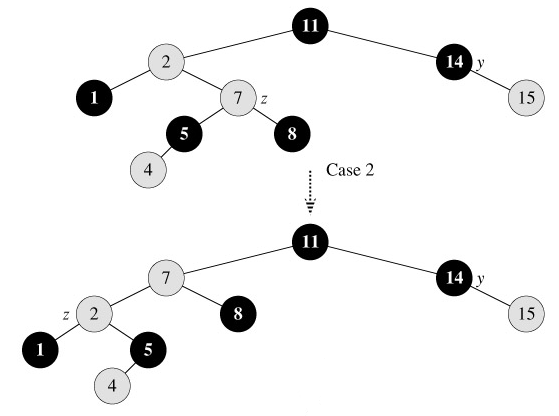
\includegraphics[width=\textwidth]{11.2}
		 \caption{Broken \hyperref[itm:red-black-tree-property4]{Red-Black Property \#4}: Case \#2}
		 \label{fig:red-black-insert-case-2}
	 \end{figure}
\end{minipage}\hfill
\begin{minipage}{0.5\textwidth}
	Node $Z$ is a right child and its parent is red and its uncle is NOT red.\\
	Do a single rotation, preserving the black height property at all nodes.
	\begin{itemize}
		\item Rotate left on parent of $Z$.
		\item Re-label old parent of $Z$ as $Z$ and continue to \hyperref[fig:red-black-insert-case-3]{case \#3}.
	\end{itemize}
\end{minipage}\\\\
\begin{minipage}{0.45\textwidth}
	 \begin{figure}[H]
		 \centering
		 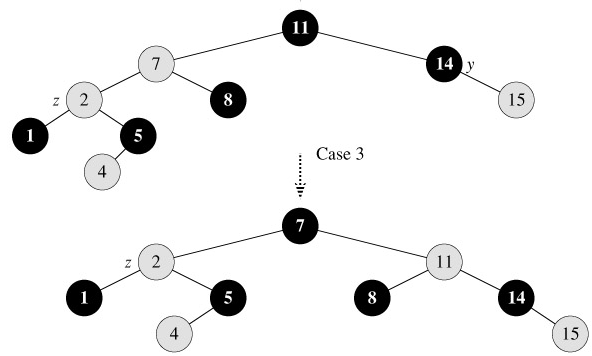
\includegraphics[width=\textwidth]{11.3}
		 \caption{Broken \hyperref[itm:red-black-tree-property4]{Red-Black Property \#4}: Case \#3}
		 \label{fig:red-black-insert-case-3}
	 \end{figure}
\end{minipage}\hfill
\begin{minipage}{0.5\textwidth}
	Node $Z$ is a left child and its parent is red and its uncle is NOT red.\\
	Do a single rotation and swap the colors of a parent node and both its children, preserving the black height property at all nodes.
	\begin{itemize}
		\item Rotate right on grandparent of $Z$
		\item Color old parent of $Z$ black
		\item Color old grandparent of $Z$ red
	\end{itemize}
\end{minipage}
%</Lecture-Activity-11>

\end{document}